\chapter{Configuration Layout \& System Characteristics}
\label{ch:configuration_layout}

\todo[inline]{From the \textit{Project Guide}:\\
The configuration / layout shows the physical appearance of the product or system. It is mainly a set of sketches and drawings illustrating the internal and external layout with a short textual
explanation. The layout contains also a block diagram identifying the electronic units carried on-board.\\
A first version is presented in the Mid Term Report, generally for all design options involved in the concept selection, concentrating on those aspects that are essential to provide the trade-off.\\
The final, more detailed, version of the final design is included in the Final Report.}

\todo[inline]{Chapter introduction pending. Remember to connect it to the previous chapters.}

This chapter outlines the structure of the external and internal layout of HUGO, emphasising the components needed to achieve research missions and their location within the airframe. \autoref{sec:resource_allocation_budget_breakdown} presents the resource allocation and budget breakdown, identifying the key budgets that constrain the dimensional requirements of the fuselage and wings and describing the methodology used for their definition and allocation.
Once the available resources are identified and quantified, \autoref{sec:external_configuration} goes into more detail regarding the outside characteristics of the frame, including the placement of the landing gear, outside sensors, instruments and landing gear. Moving towards the internal components, \autoref{sec:internal_configuration} outlines the systems that keep HUGO alive and functioning, such as the electronics, power system and sensors. Once all the details that give life to HUGO have been identified, the design team can move further towards analysing the performance of the flights.

\section{Resource Allocation \& Budgets}
\label{sec:resource_allocation_budgets}
- identify the key budgets (reference baseline report?)
- describe how they drive the design + values

\subsection{Centre of Gravity Location}
% - center of gravity
%     *explain that we aimg at having a range for the cg so that we can test for both the stable and unstable configuration
%     *we aim at testing via movement of the fuel from the bladders by the use of a reversable pump that is connected between the 2 bladders
%     *here we can explain that the test will be further explained in the section with the tests and so on so we dont go to much in detail 
%     *we mention that the cg can be varied with the aid of the fuel tanks, wings and tail
The centre of gravity was identified in an earlier analysis (during the baseline report) as a resource that must be taken into account to meet the stability requirements. While considering possible test scenarios, it was concluded that in the event of a stability experiment, an elegant way to shift the location of the CG is to vary the distribution of the fuel between two reservoirs. This method will further be emphasised in \todo{add the citation once the section for experiments is written}.

Internal elements such as the electronic and propulsion systems are the main drivers of the CG location, along with the structure itself. In this phase, it was decided to go with a segmented approach regarding the determination of the CG position by separating the gravity centre of the fuselage from the centre of the components. The electronic and propulsion system are sized and thier elements positioned inside the plane, giving the design team an initial location of CG that the fuselage and the wings can use as referance. The advantage of this method is that during the iteration process, the CG can be shifted by moving components of the mentioned systems inside the fuselage.

Aiming at having a client base that brings its own wings to the test site and can configure HUGO to meet their internal arrangements, which means the CG range has a large variation. Moreover, the tests include experiments where the plane has to perform in unstable variations, as such, it has been decided to not to allocate a budget to the CG of the plane, but to perform for each HUGO configuration a CG analysis and simulation.

\subsection{Communication Link Budget}
-we have the communication link from the electronic ship that is good about 200 km, we have the antenna that I forgot to add....
-we cannot use the normal comunicatin for those speeds and due to the Doppler effect that makes the signal freq be 4 times higher or lower at mach 0.75, as such we use a custom C2 communication link--> I have to explain this new communication because of the speed 
OK LETS DO THIS


\begin{itemize}
    %\item Centre of gravity location (CG location)
    \item Communication link budget
    \item Mass
    \item Aircraft dimensions
    \item Internal dimensions
    %\item Thrust
    \item Fuel budget
    \item Power from the battery
\end{itemize}


\section{External Configuration}
\label{sec:external_configuration}

- hatches, mounted sensors, 

\subsection{Landing Gear Design}
\label{sub:landing_gear_design}
- landing gear section

\subsection{Environmental Control}
\label{sub:environmental_control}
- environmental control



\section{Internal Configuration}
\label{sec:internal_configuration}
%- a brief description of systems that go inside (electronic, propulsion, sensors)
%- tables of sensors, their purpose, and location
- figures of configs for different missions (autoref ops \& logistics)
    idea: figures for one config in this chapter, the rest in the appendix

\subsection{Electronics System Design}
\label{sub:electronics_system_design}

- section about electronic system
\autoref{fig:electronics_mapping} shows the interactions between electronics system components in terms of power, signal, and fuel flow.

\begin{figure}[H]
    \centering
    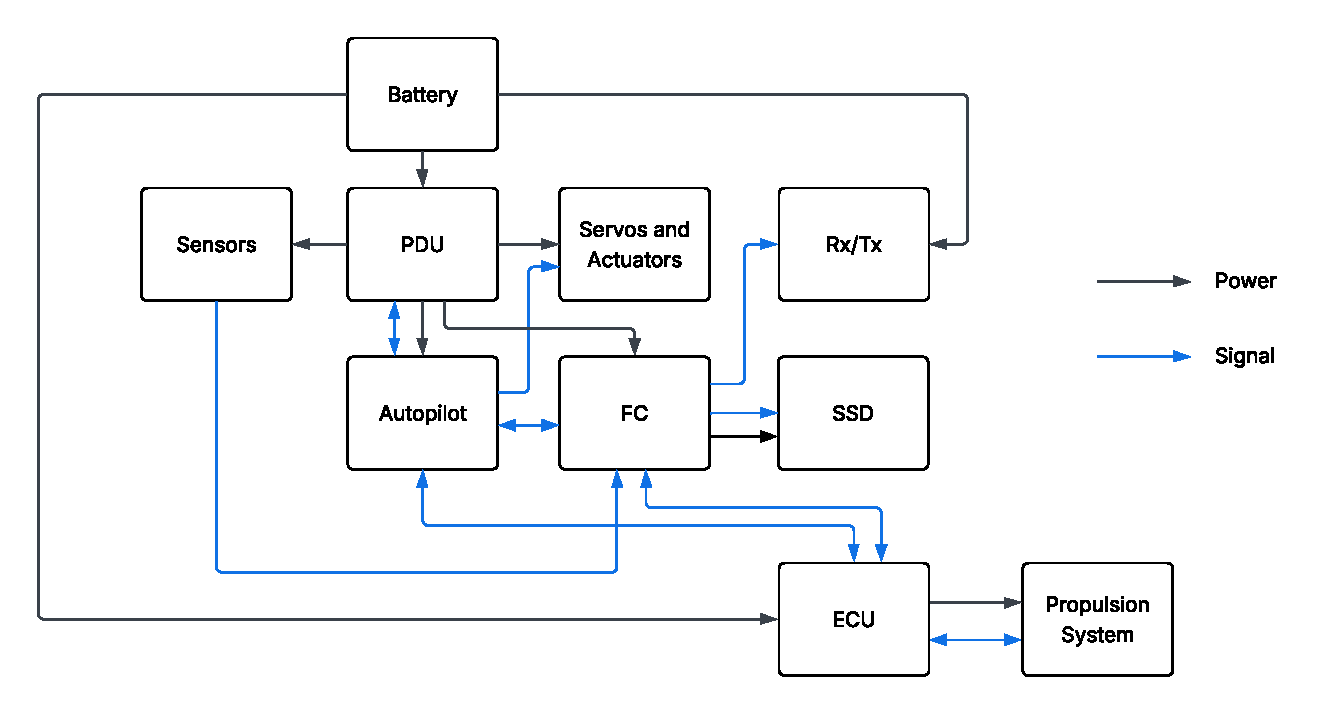
\includegraphics[width=1\linewidth]{figures_final/electronic_system.pdf}
    \caption{Electronics system mapping}
    \label{fig:electronics_mapping}
\end{figure}


\subsection{Propulsion System Design}
\label{sub:propulsion_system_design}
- section about propulsion system (think we can take it from the midterm for this one\\
\autoref{fig:fuel_system_mapping} showcases the interaction between propulsion system components in terms of power, signal, and fuel flow.


\begin{figure}[H]
    \centering
    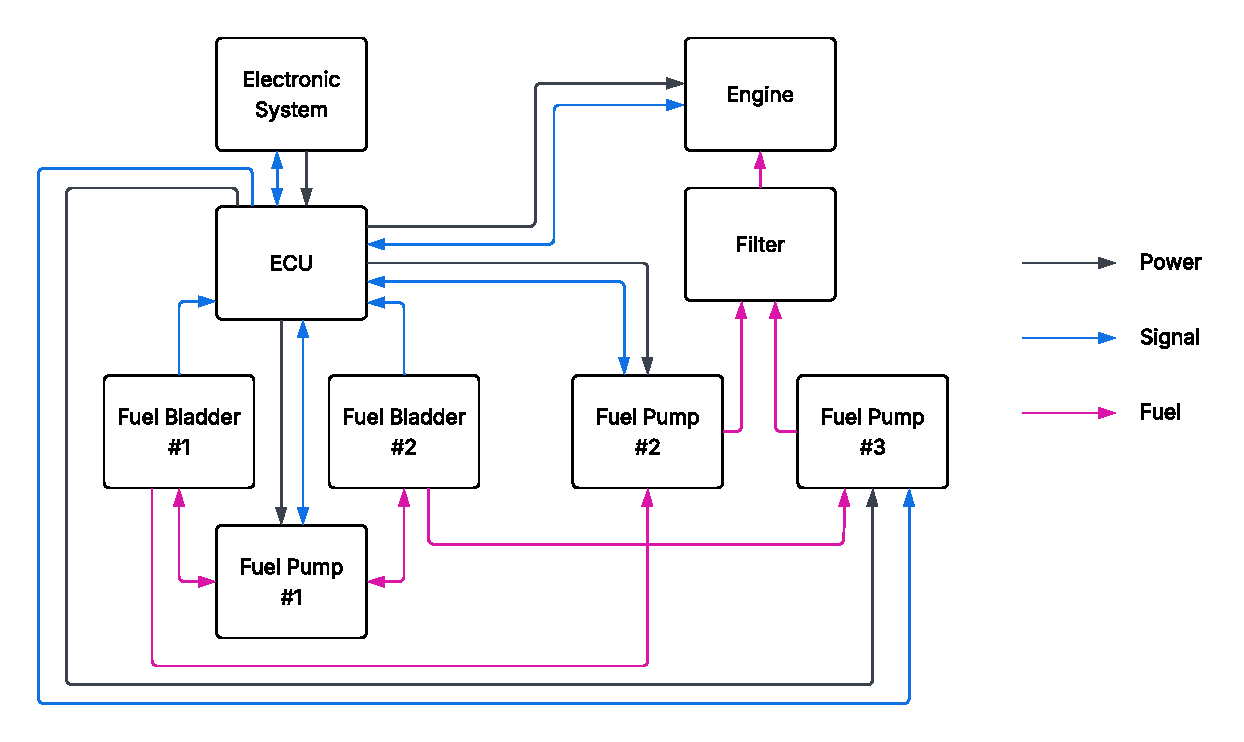
\includegraphics[width=1\linewidth]{figures_final/fuel_system.pdf}
    \caption{Propulsion system mapping}
    \label{fig:fuel_system_mapping}
\end{figure}


\subsection{Sensor Interaction}
\label{sub:sensor_interaction}
- list of sensors for different test cases (autoref ops \& logistics)\\
- section about the sensors and how they communicate (diagram)\\



\begin{longtable}{|c|p{3cm}|p{5cm}|p{3cm}|p{2cm}|}
        \caption{Sensors used for test measurements}
        \label{tab:internal_config_test_measurement_sensors}\\
\hline
       \textbf{Sensor ID} & \textbf{Sensor} & \textbf{Description} & \textbf{Dimensions [m]} & \textbf{Weight [kg]} \\\hline
\endfirsthead
\hline
\textbf{Sensor ID} & \textbf{Sensor} & \textbf{Measurement type} & \textbf{Dimensions [m]} & \textbf{Weight [kg]} \\\hline
\endhead
\hline
\multicolumn{5}{r}{\textit{Continued on next page}} \\
\endfoot
\hline
\endlastfoot
        HUG-SEN-01 & FBG sensor \footnote{\href{https://www.peraglobe.com/robust-flight-qualified-fbg-interrogator}{FBG} (accessed on 01.06.2026)}& Wing deflection & $0.150 \times 0.125 \times 0.0585$  & 0.700\\\hline
        HUG-SEN-02 & Load-cell & Wing surface strain & & \\\hline
        HUG-SEN-03& Strain rosetta  & Strain & & \\\hline
        HUG-SEN-04& LIDAR-sensor & Weather detection, wing deflection & $0.35\times 0.35\times0.15$ &  \\\hline
       HUG-SEN-05 & Camera\footnote{\href{https://www.phaseone.com/wp-content/uploads/2024/01/P5_Brochure_Display_EN_2023.pdf}{PhaseOne} (accessed on 01.06.2026)}  & Deflection, Visual inspection of structural behavior & $0.075 \times 0.075 \times 0.09$ & 0.700 \\\hline
        HUG-SEN-06& Pitot probe  & Airspeed & & \\\hline
       HUG-SEN-07 & Gyroscope  & Attitude & & \\\hline
       HUG-SEN-08 & Accelerometer  & Acceleration & & \\\hline
        HUG-SEN-09& Altimeter  & Altitude & & \\\hline
        
\end{longtable}

- sketches for different mission examples (in the appendix)







\todo[inline]{Chapter conclusion pending. Remember to connect it to the chapters that come after.}